\chapter{Conflitos de Controlo}
A unidade de Conflitos de Controlo analisa as instruções que chegam ao andar de \textit{Instruction Decoding/Register Fetch} e em caso de se tratar de uma instrução de transferência de controlo decide o próximo endereço a colocar no registo do \textit{Program Counter}.\\

As instruções de transferência de controlo dividem-se em 3 formatos:\\

\section{Formato I}
\begin{table}[H]
	\centering
	\begin{tabular}{cccccccccccccccc}
		15 & 14 & 13 & 12 & 11 &  &  & 8 & 7 &  &  &  &  &  &  & 0 \\ \hline
		\multicolumn{1}{|c}{0} & \multicolumn{1}{c|}{0} & 0 & \multicolumn{1}{c|}{0} & \multicolumn{4}{c|}{Cond} & \multicolumn{8}{c|}{Destino} \\ \hline
		\multicolumn{1}{|c}{0} & \multicolumn{1}{c|}{0} & 0 & \multicolumn{1}{c|}{1} & \multicolumn{4}{c|}{Cond} & \multicolumn{8}{c|}{Destino} \\ \hline
	\end{tabular}
\end{table}
Para este formato é usada uma BTB onde são armazenados os dados para prever o resultado \\
Para executar a predição dos saltos são usados 2 bits que codificam 4 estados, onde o bit mais significa é usado para decidir entre saltar e não saltar.
\begin{table}[H]
	\begin{tabular}{ll}
		$00$ & strong not taken	\\
		$01$ & weak not taken	\\
		$10$ & weak taken		\\
		$11$ & strong taken
	\end{tabular}
\end{table}
Esta predição é depois atualizada com os resultados da unidade de flags e com a utilização de uma BPB e armazenada esta nova informação na BTB.

\section{Formato II e III}
No caso dos Formatos II e III não existe a necessidade de fazer predição, pois tratam-se de saltos incondicionais, ou seja, ocorrem sempre.\\

No caso do Formato II é um salto com um offset e é usado um somador na própria unidade de Conflitos de Controlo.
\begin{table}[H]
	\centering
	\begin{tabular}{cccccccccccccccc}
		15 & 14 & 13 & 12 & 11 &  &  &  &  &  &  &  &  &  &  & 0 \\ \hline
		\multicolumn{1}{|c}{0} & \multicolumn{1}{c|}{0} & 1 & \multicolumn{1}{c|}{0} & \multicolumn{12}{c|}{Destino} \\ \hline
	\end{tabular}
\end{table}
No caso do Formato III é um salto para um valor armazenado num registo RB, valor este que é verificado pela unidade de Conflito de Dados se o valor presente no Register File é o mais atualizado ou se há a necessidade de fazer forwarding.
\begin{table}[H]
	\centering
	\begin{tabular}{cccccccccccccccc}
		15 & 14 & 13 & 12 & 11 & 10 &  &  &  &  &  &  & 3 & 2 &  & 0 \\ \hline
		\multicolumn{1}{|c}{0} & \multicolumn{1}{c|}{0} & 1 & \multicolumn{1}{c|}{1} & \multicolumn{1}{c|}{R} & \multicolumn{8}{c|}{} & \multicolumn{3}{c|}{RB} \\ \hline
	\end{tabular}
\end{table}

\section{BTB}
A BTB consiste numa pequena memória que funciona como \textit{cache} que armazena os resultados de ocorrências passadas da mesma instrução e qual o seu desfecho.
A BTB tem 128 posições endereçadas pelos 7 bits menos significativos do PC da instrução de controlo e os restantes bits são armazenados como uma TAG que é usada para verificar se a instrução em memória corresponde à mesma transferência controlo.\\

É também armazenados os bits de predição que ajudam a determinar se o salto vai ser \textit{taken} ou \textit{not taken}.

\section{BPB}
A BPB consiste numa unidade que recebe os bits de predição antigos e o verdadeiro resultado da instrução proveniente da unidade de flags e calcula os bits atualizados.
\begin{table}[H]
	\centering
	\begin{tabular}{cc|c|cc}
		\multicolumn{2}{c|}{Old bits} & Taken & \multicolumn{2}{c}{New bits} \\ \hline
		0 & 0 & 0 & 0 & 0 \\
		0 & 0 & 1 & 0 & 1 \\
		0 & 1 & 0 & 0 & 0 \\
		0 & 1 & 1 & 1 & 0 \\
		1 & 0 & 0 & 0 & 1 \\
		1 & 0 & 1 & 1 & 1 \\
		1 & 1 & 0 & 1 & 0 \\
		1 & 1 & 1 & 1 & 1
	\end{tabular}
\end{table}
Estes novos bits são armazenados na BTB para serem usados em próximas ocorrências da instrução.


\begin{figure}[H]
	\begin{center}
		\makebox[\textwidth][c]{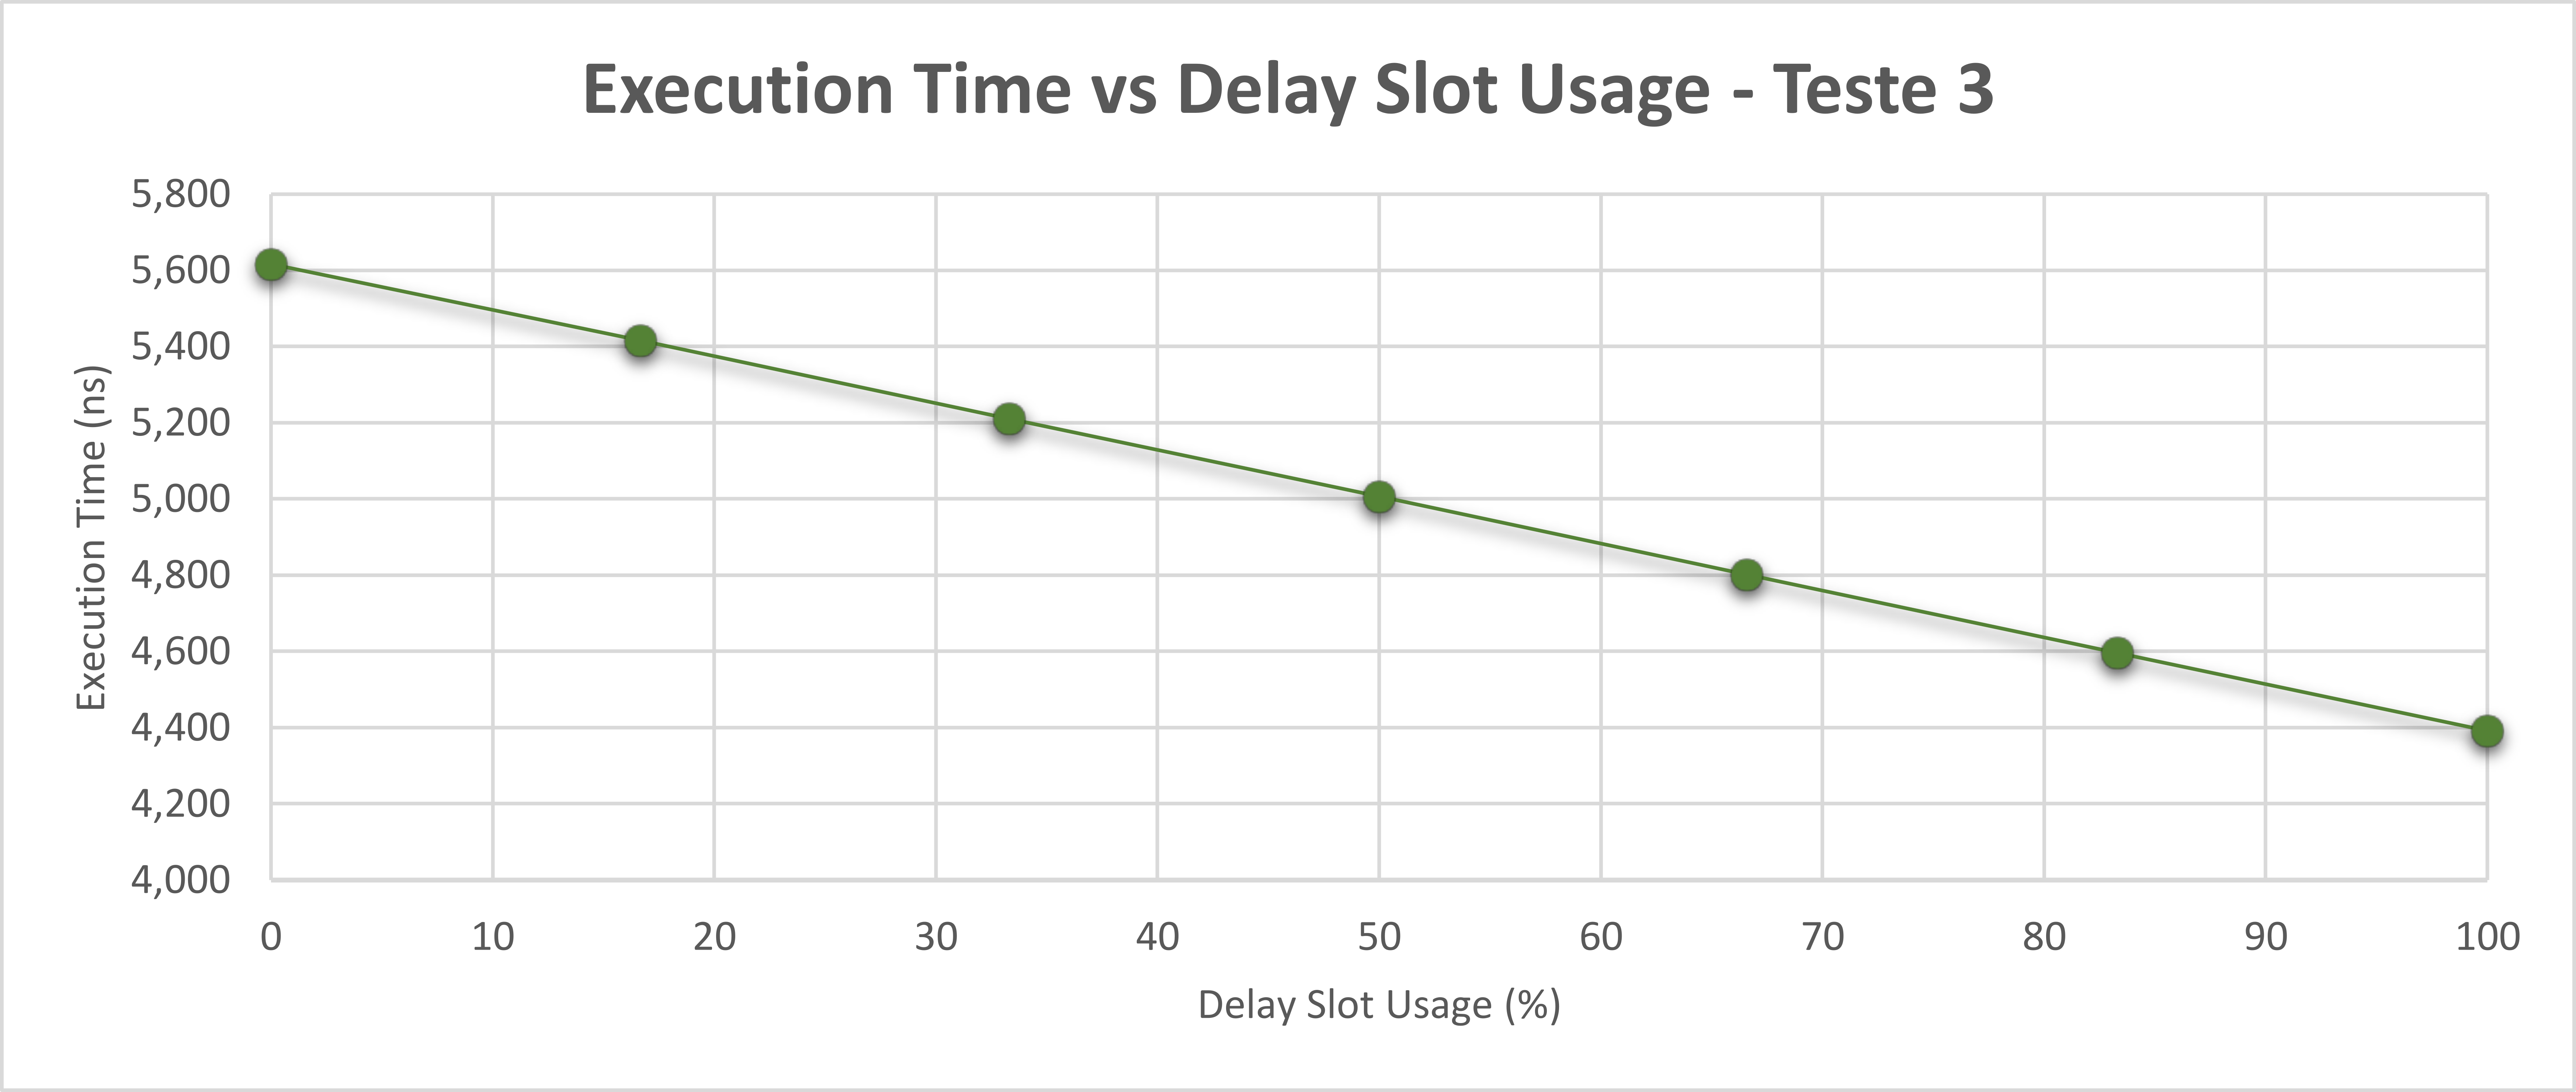
\includegraphics[clip, keepaspectratio=true, scale=1]{./images/path9919.png}}
		\caption{Relação Tempo de execução - Utilização do Delay Slot para Teste 3.}
		\label{tempexet3}
	\end{center}
\end{figure}

\begin{figure}[H]
	\begin{center}
		\makebox[\textwidth][c]{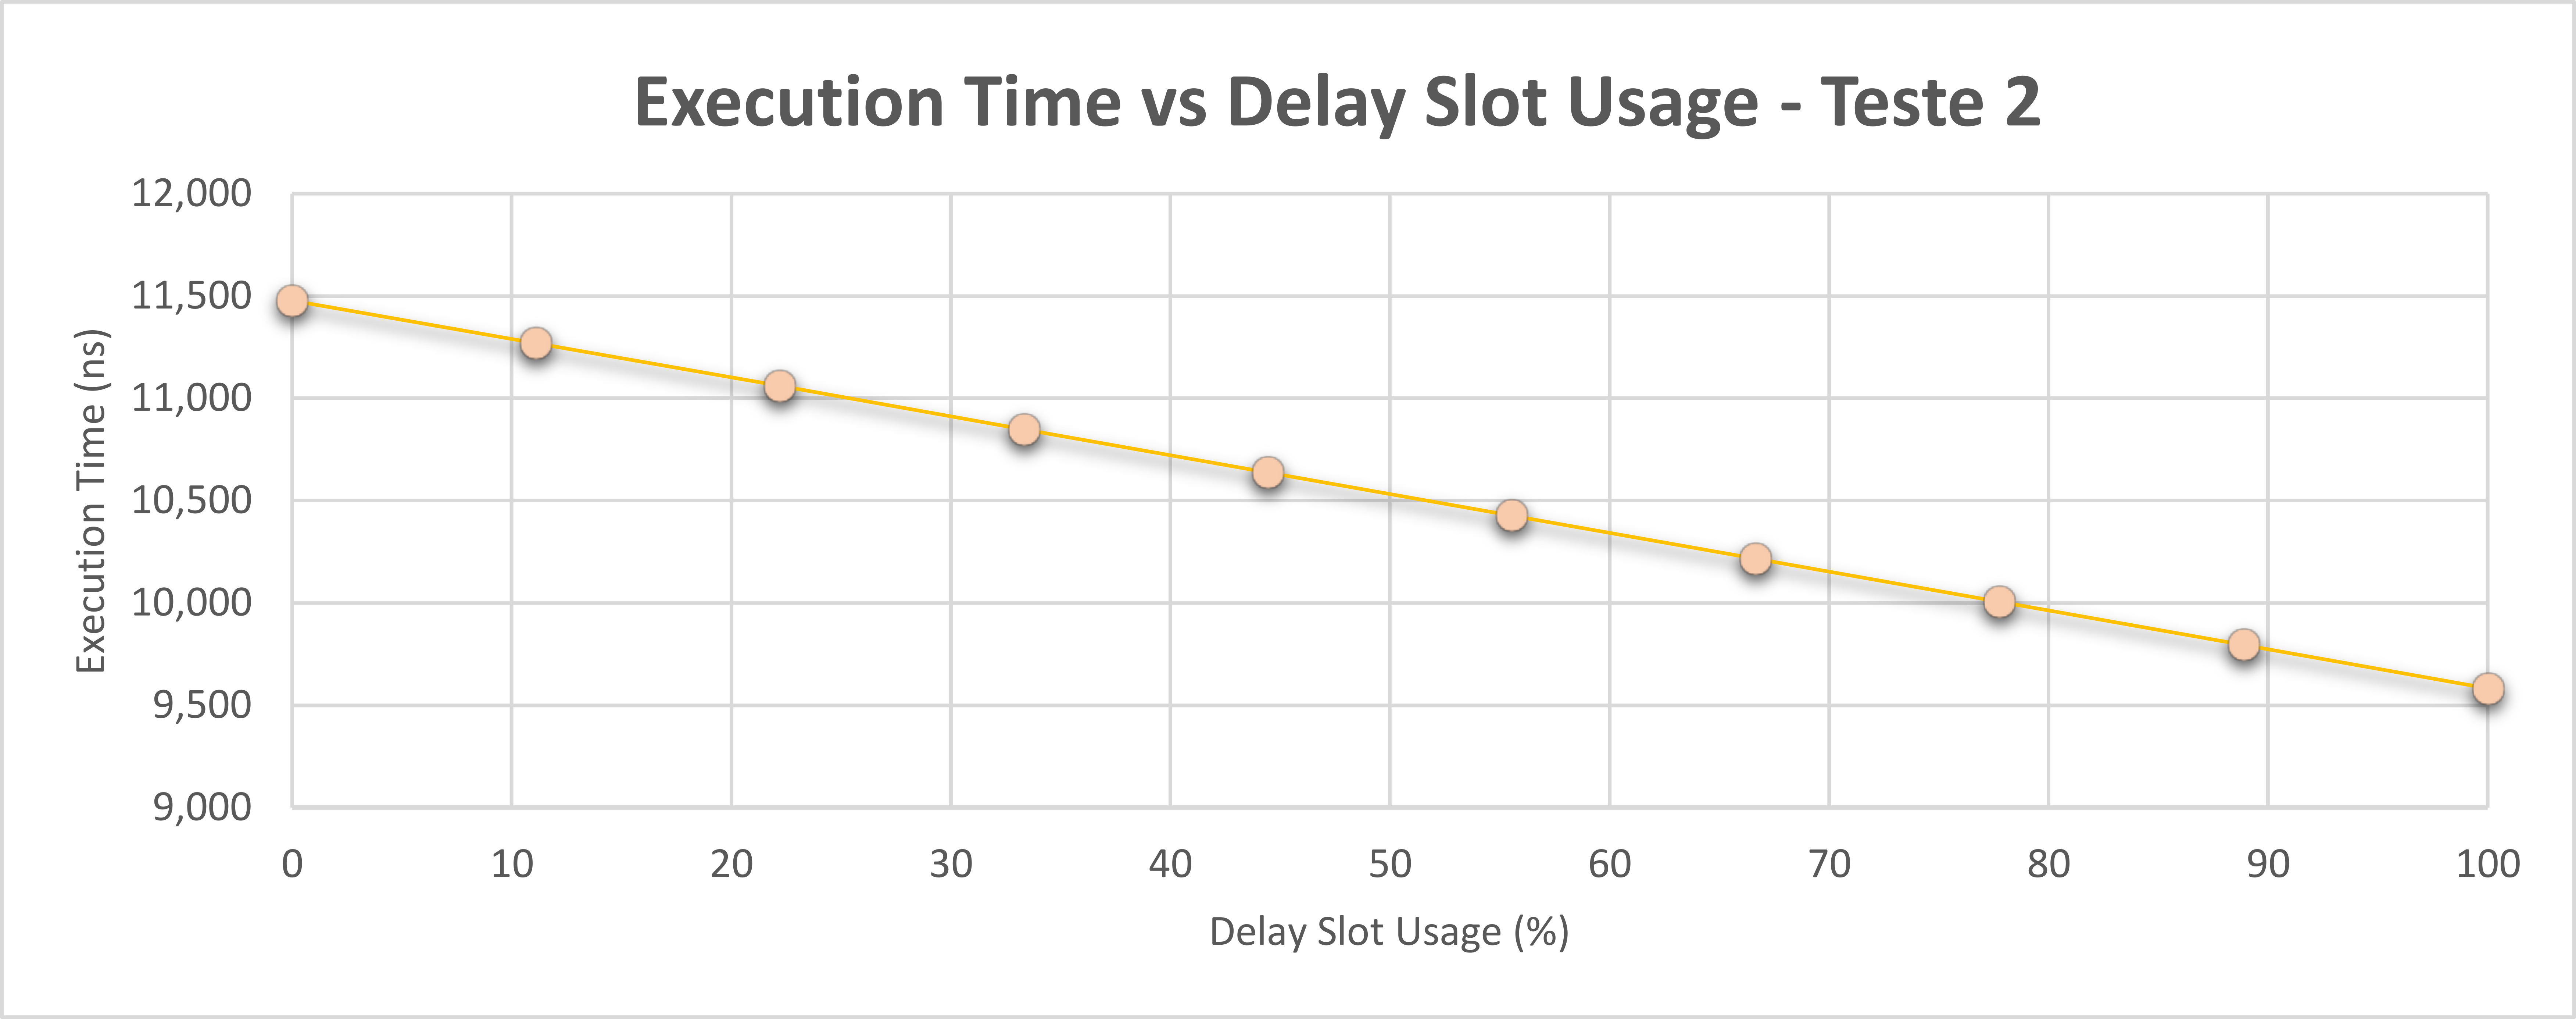
\includegraphics[clip, keepaspectratio=true, scale=1]{./images/path9347.png}}
		\caption{Relação Tempo de execução - Utilização do Delay Slot para Teste 2.}
		\label{tempexet2}
	\end{center}
\end{figure}

\begin{figure}[H]
	\begin{center}
		\makebox[\textwidth][c]{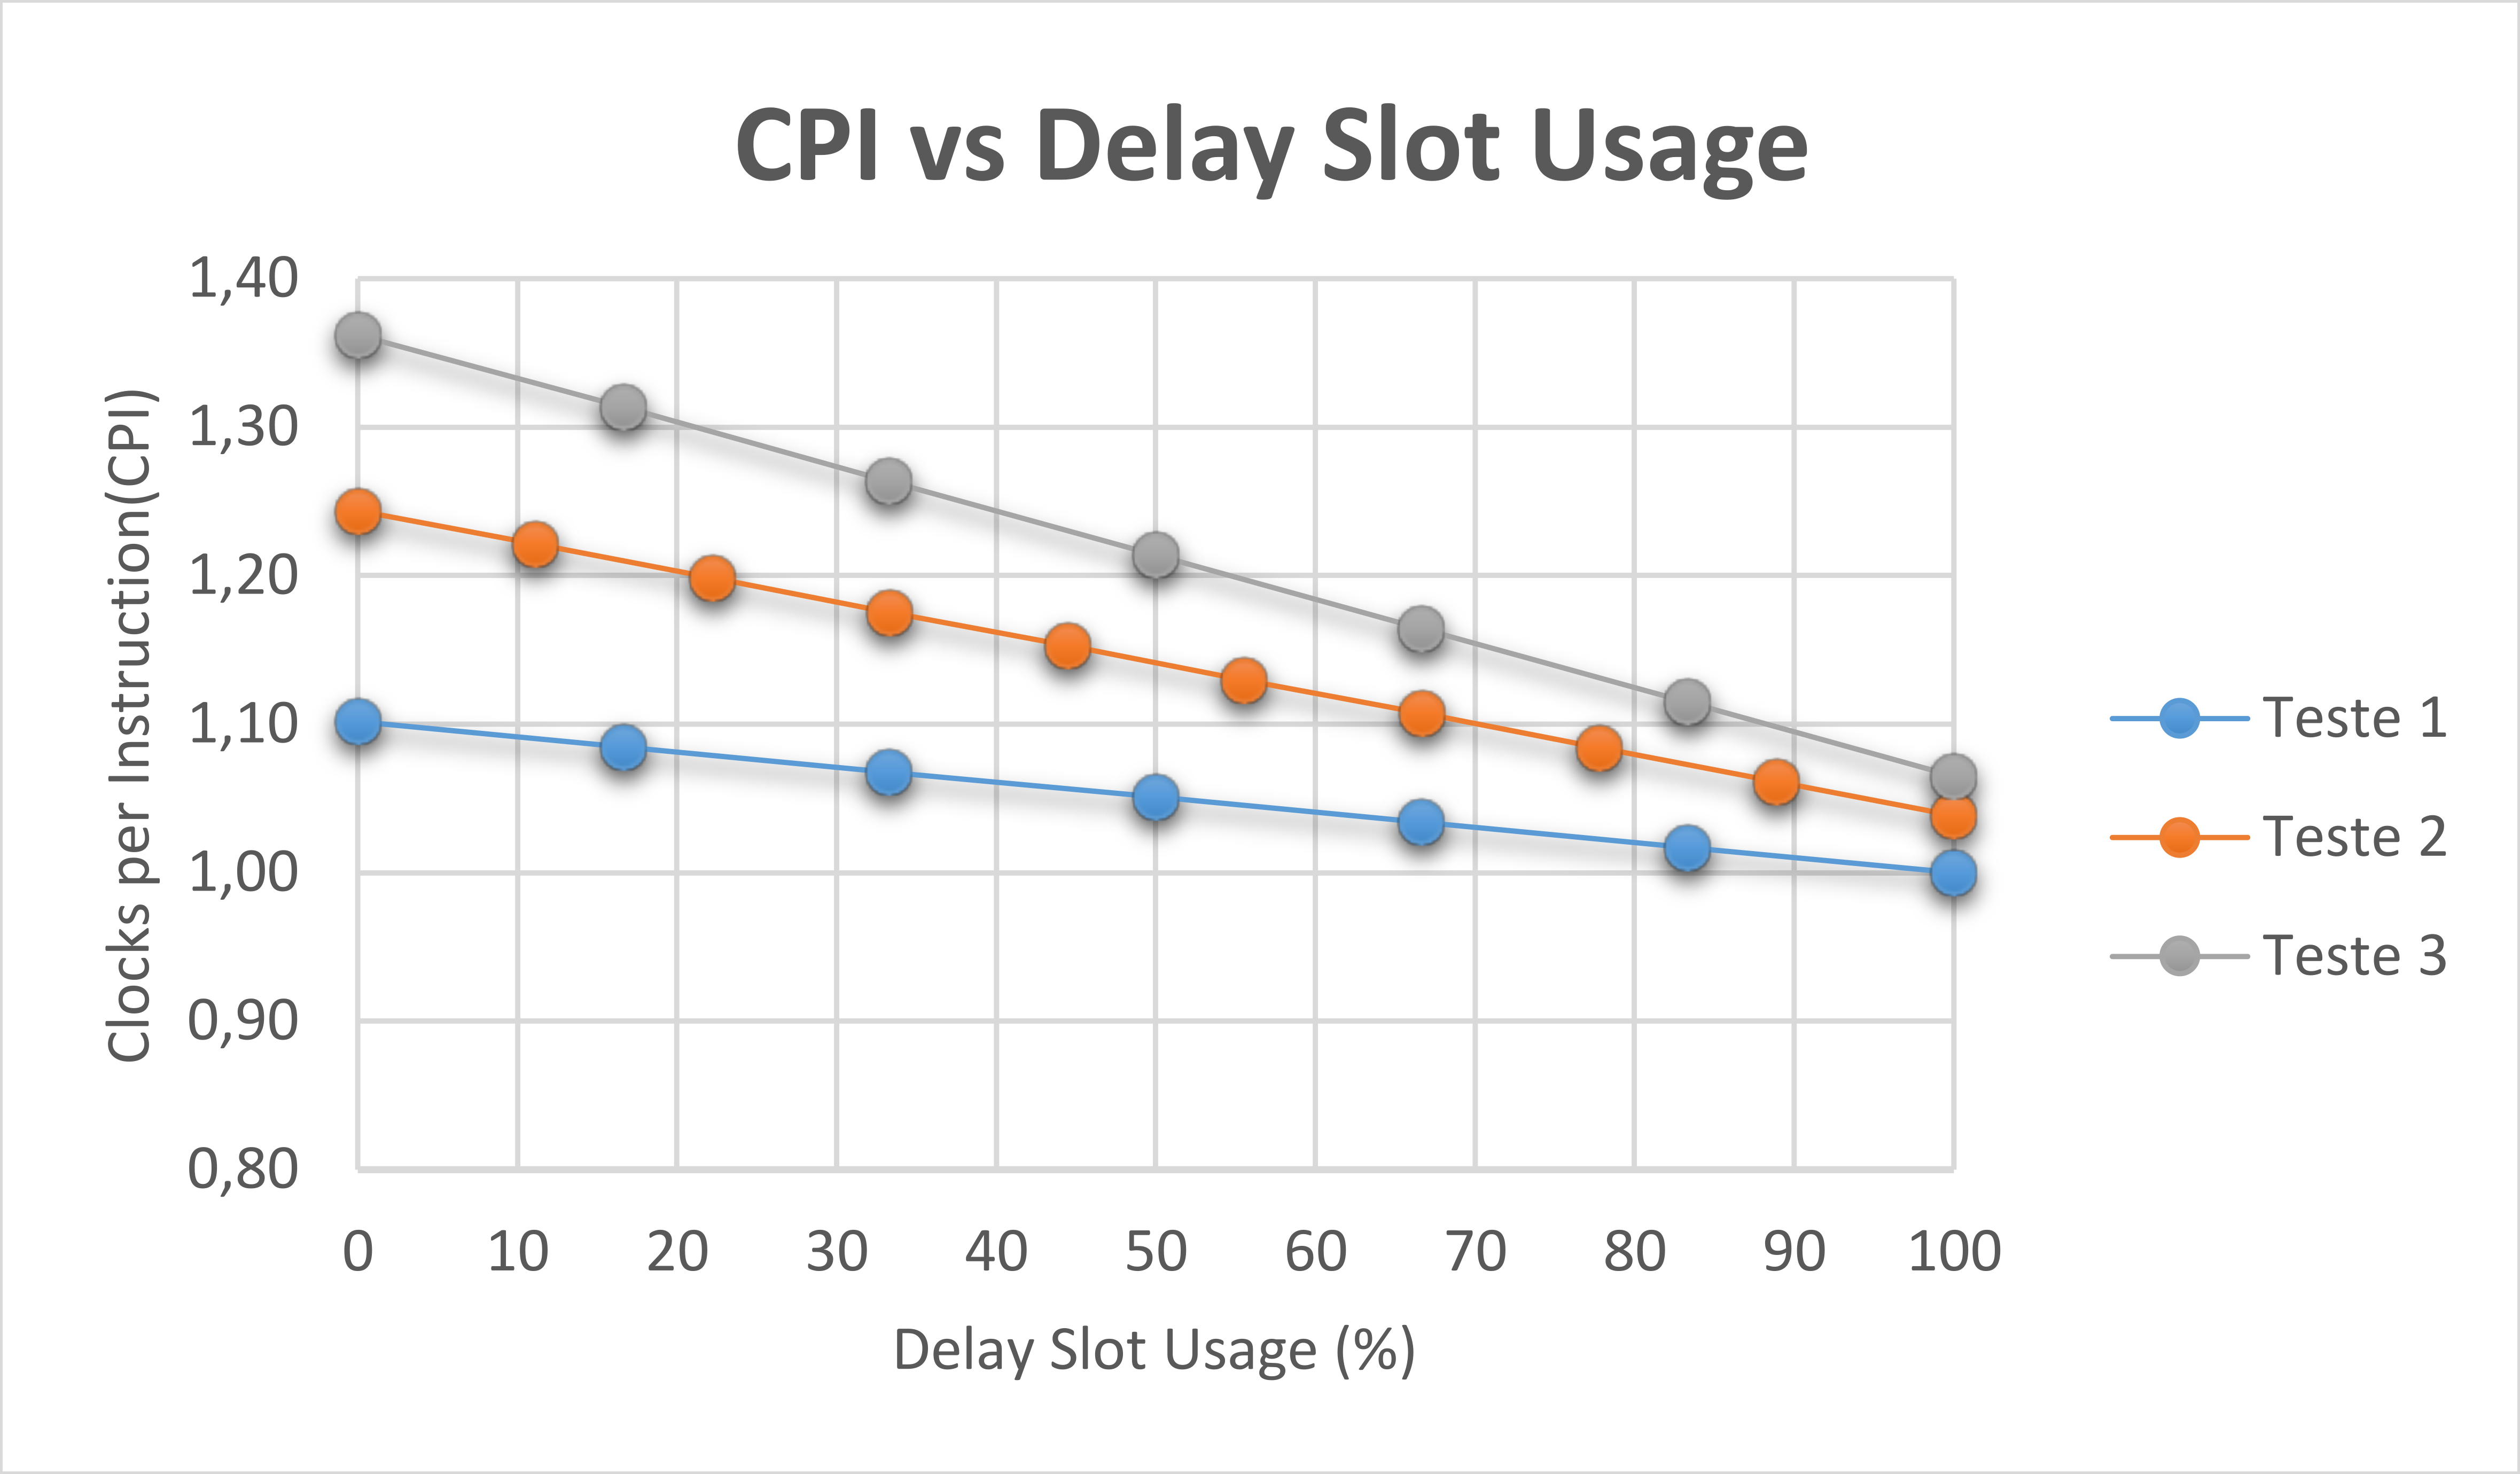
\includegraphics[clip, keepaspectratio=true, scale=1]{./images/path10881.png}}
		\caption{Relação CPI - Utilização do Delay Slot para os Testes 1,2 e 3.}
		\label{cpi}
	\end{center}
\end{figure}

\begin{figure}[H]
	\begin{center}
		\makebox[\textwidth][c]{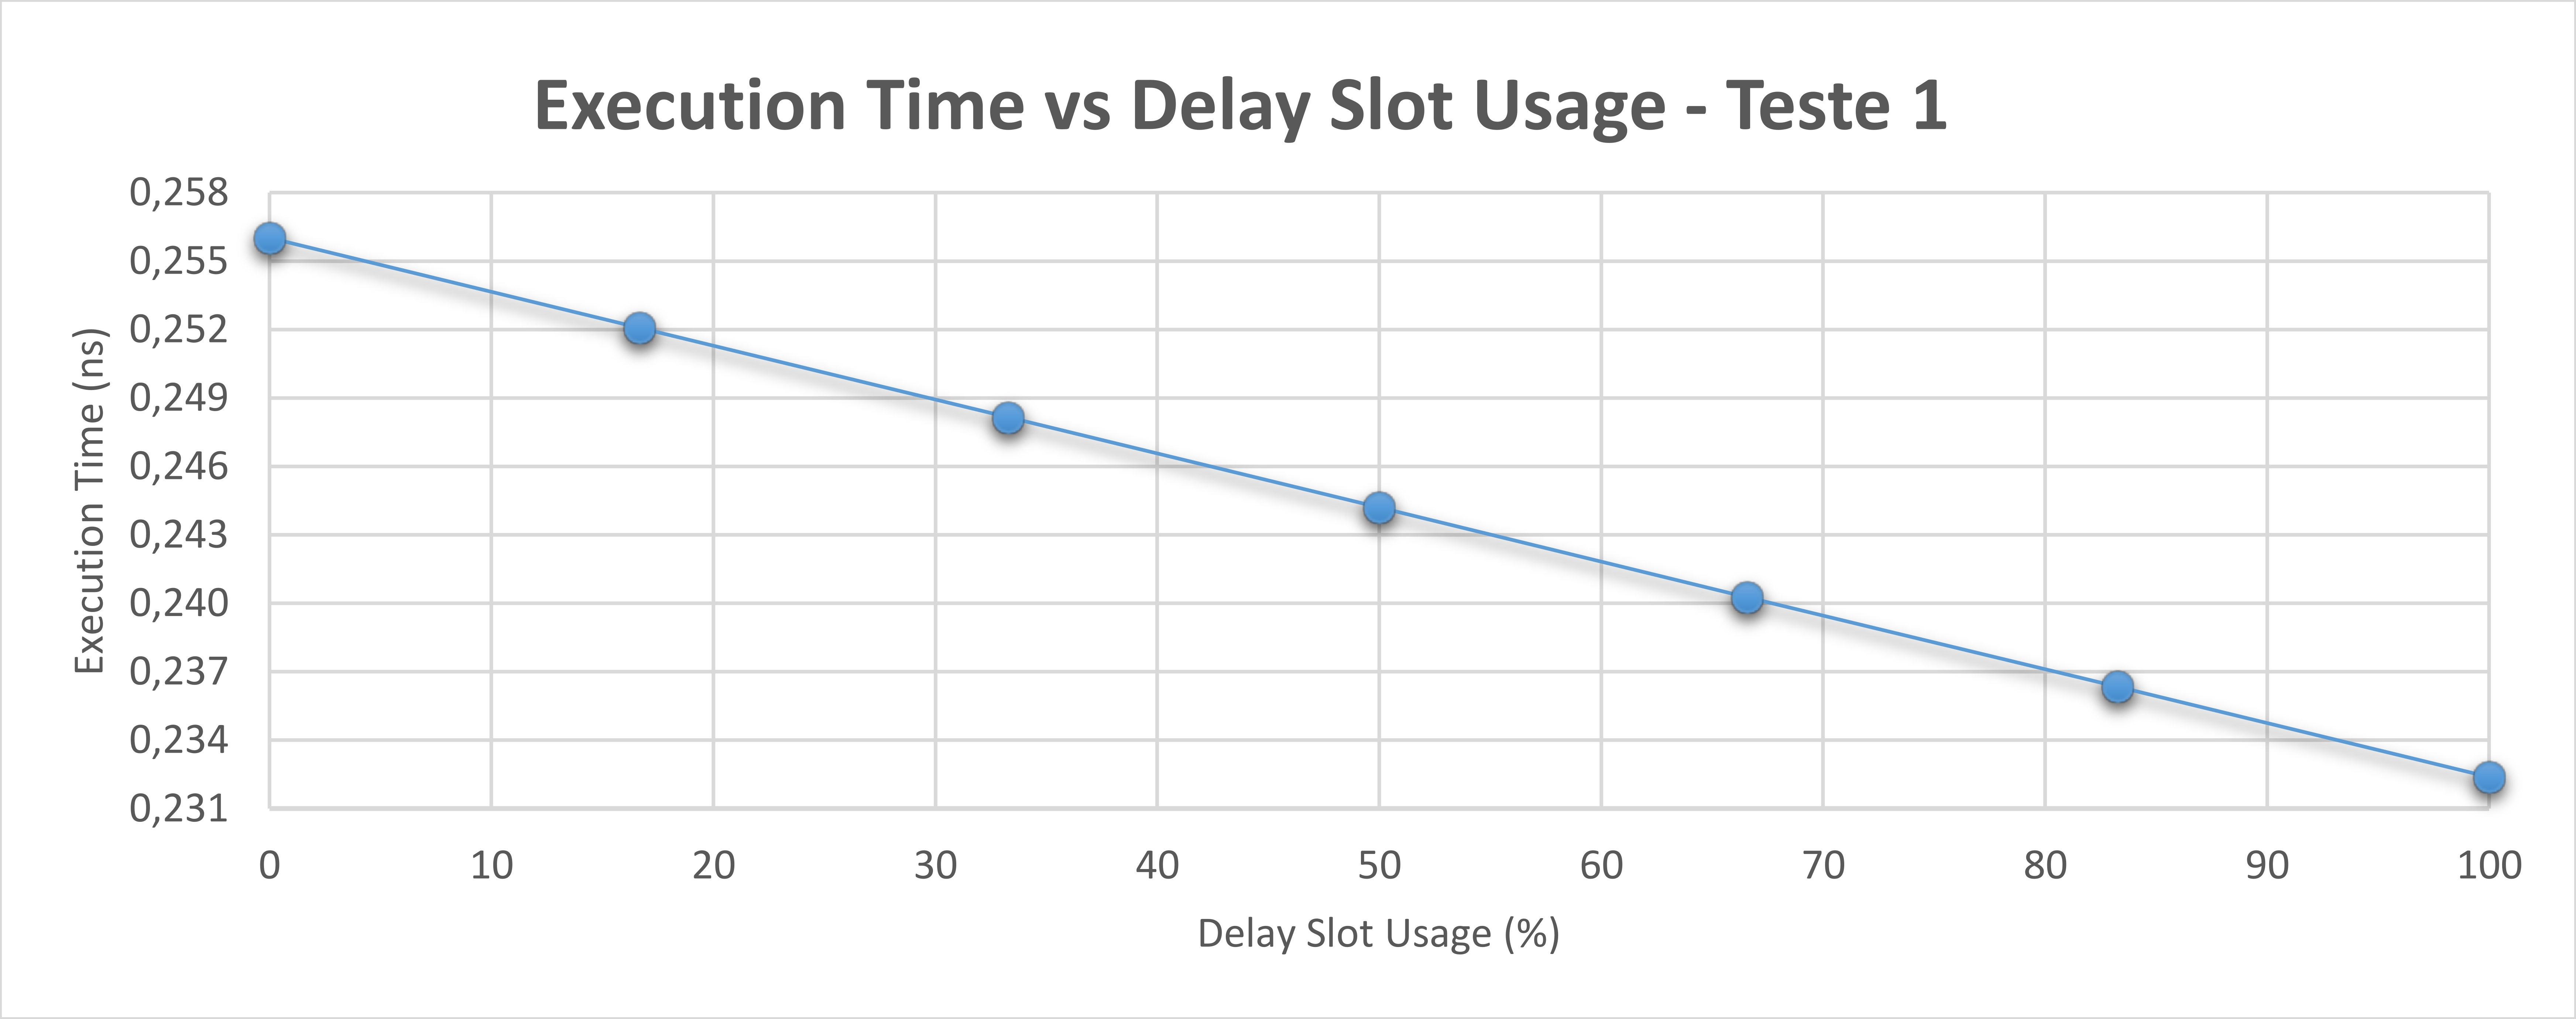
\includegraphics[clip, keepaspectratio=true, scale=1]{./images/path12085.png}}
		\caption{Relação Tempo de execução - Utilização do Delay Slot para Teste 1}
		\label{tempexet1}
	\end{center}
\end{figure}

\begin{figure}[H]
	\begin{center}
		\makebox[\textwidth][c]{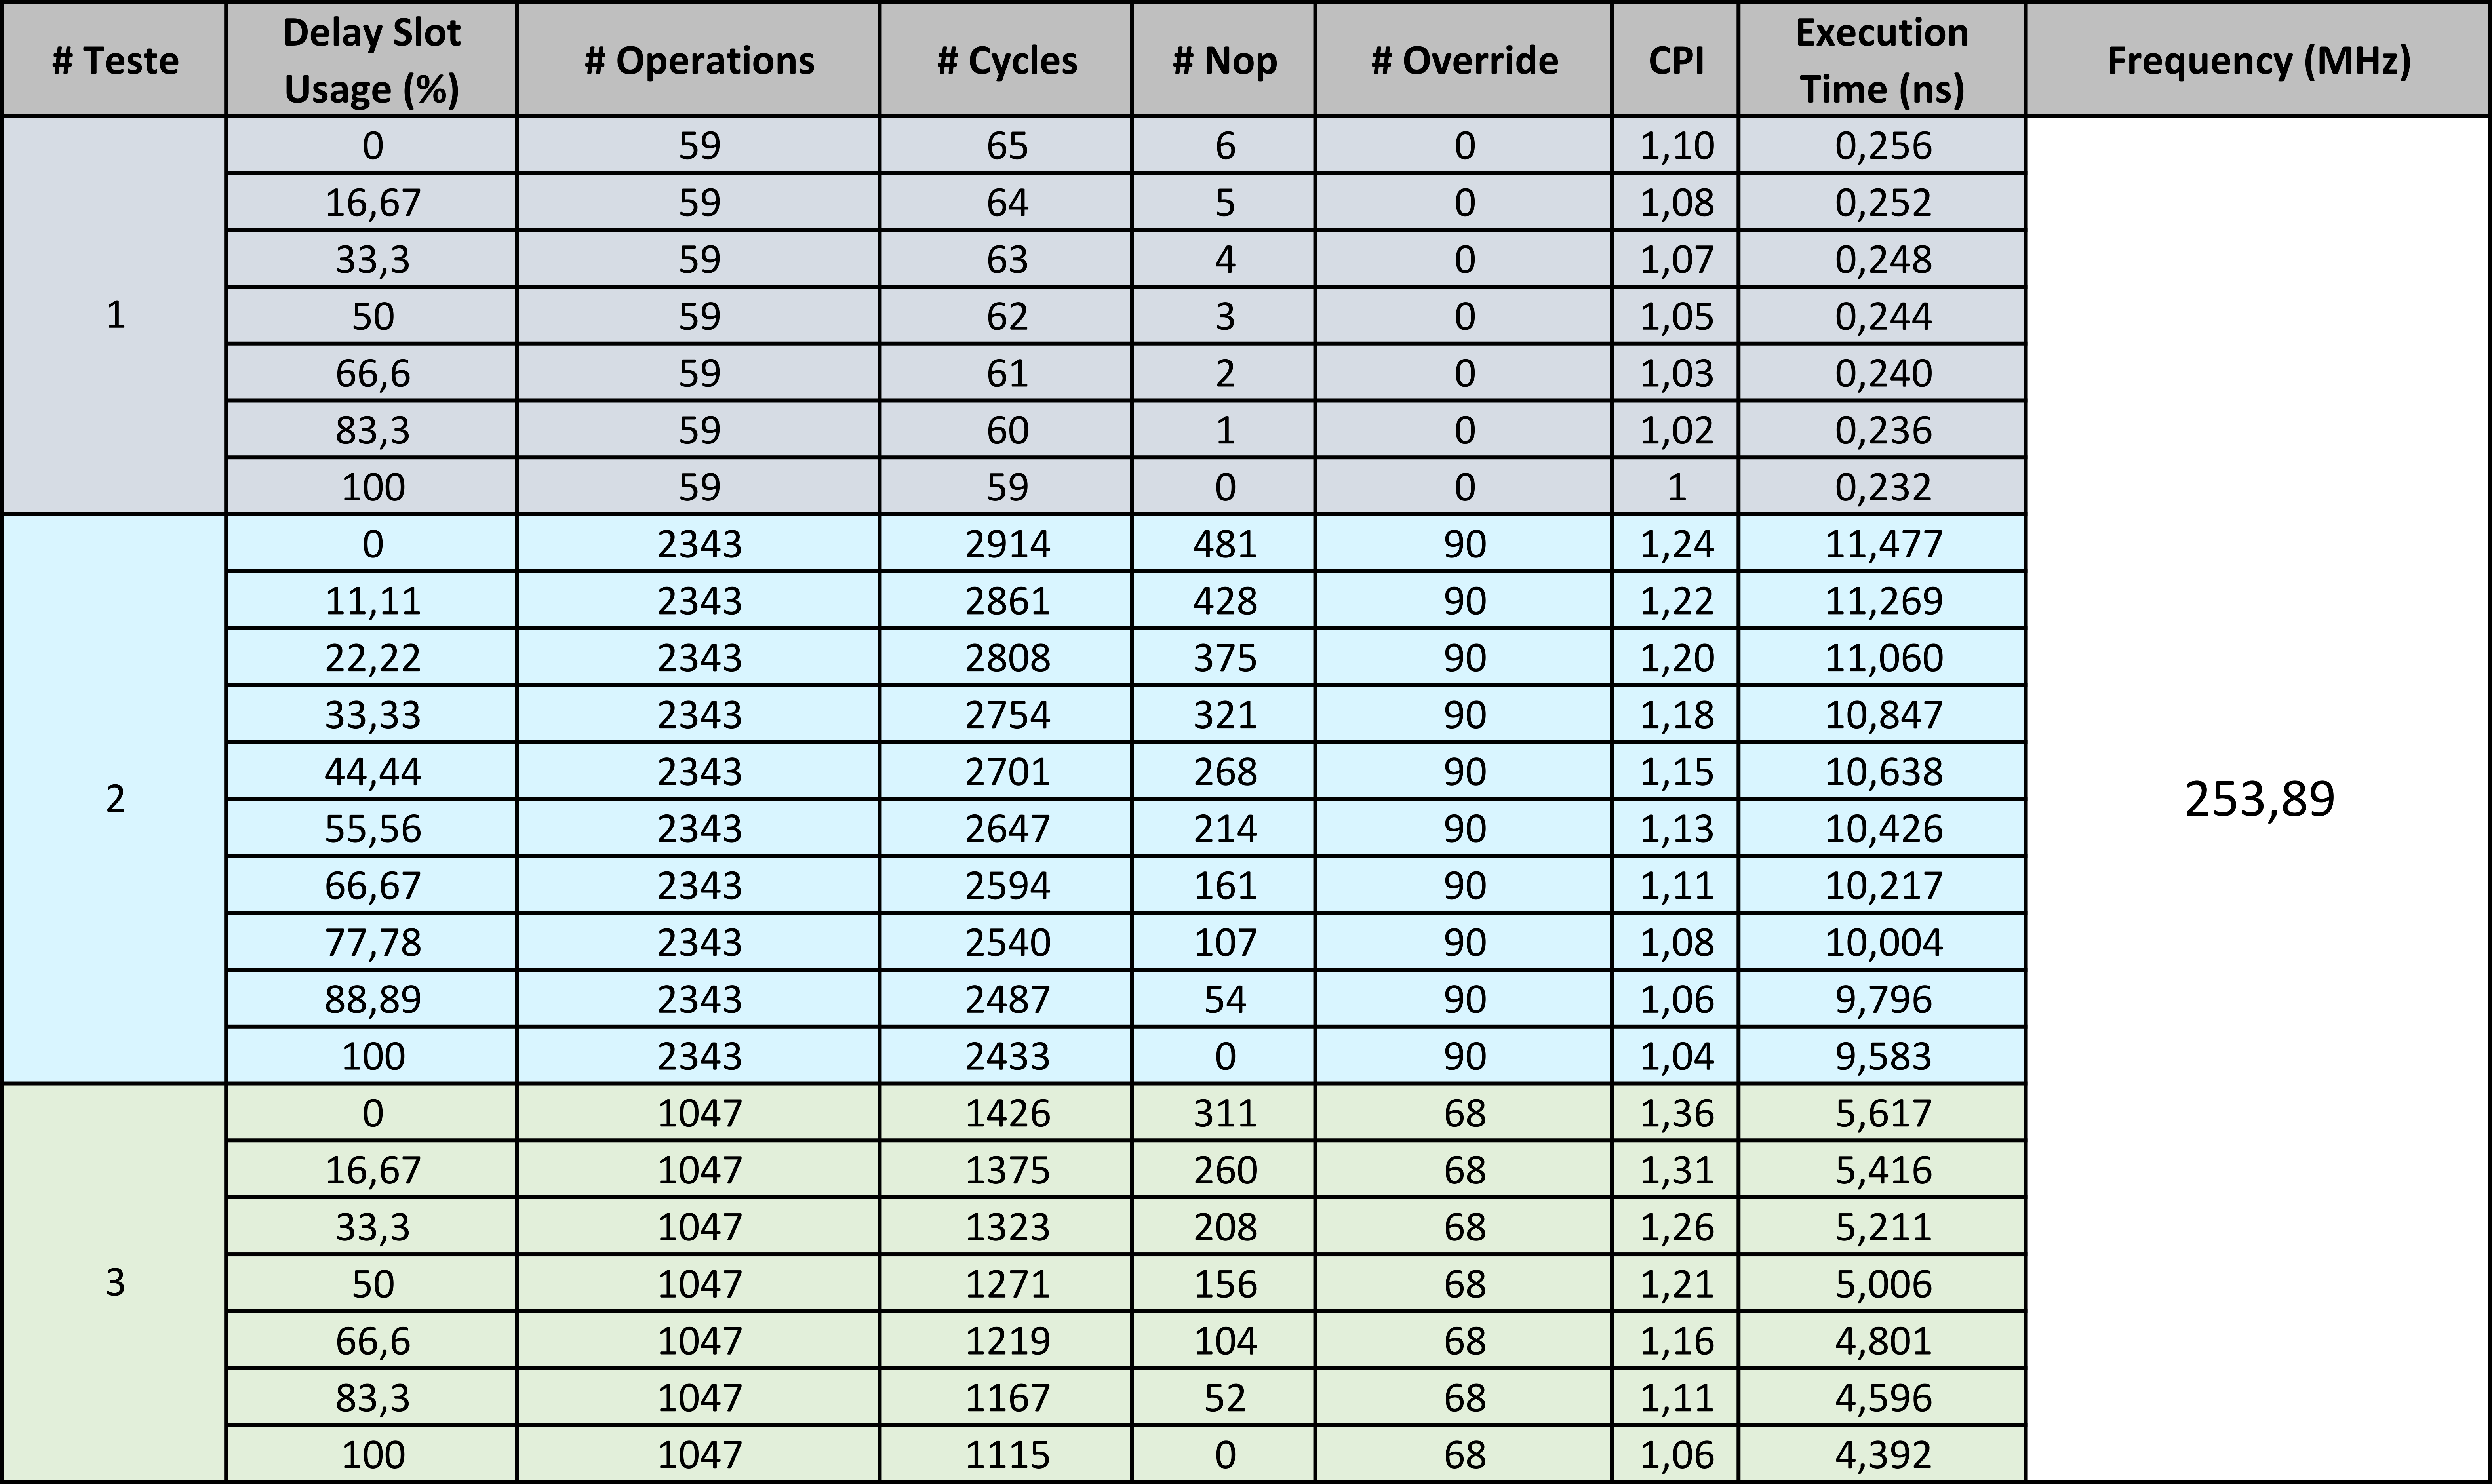
\includegraphics[clip, keepaspectratio=true, scale=1]{./images/g10791.png}}
		\caption{Estatísticas do Pipeline para os Testes realizados.}
		\label{tabela}
	\end{center}
\end{figure}